In diesem Abschnitt werden typische Abläufe von Aktionen dargestellt, die ein Anwender mit der Software durchführt. Jeder Ablauf wird mit Hilfe eines Sequenzdiagramms visualisiert. Die Diagramme stellen nur eine Übersicht auf Modulebene dar, speziellere und ggf. angepasste Sequenzdiagramme sind dem Entwurfsdokument zu entnehmen.
\par
Nachfolgend sind alle Nutzungsabläufe aus dem Pflichtenheft beschrieben, für die alle nötigen Funktionen implementiert sind. Diese wurden von einem Entwickler ausgeführt, um die korrekte Funktion gemäß des Pflichtenhefts zu überprüfen.

\section{Erzeugung eines 3D-Modells}
\textbf{Vorbedingung:} Bilder des Modells wurden erstellt. \newline
\textbf{Ergebnis:} Fertiges 3D-Modell liegt zur weiteren Verarbeitung in anderer Software vor. \newline
Der Nutzer führt folgende Schritte aus (Schritte \ref{TN3DModellBilderauswahl} bis \ref{TN3DModellSpeichern} werden in 3D-MuVi ausgeführt):
\begin{enumerate}
	\item 3D-MuVi wird gestartet.
	\item \label{TN3DModellBilderauswahl} Bilder werden ausgewählt.
	\item Algorithmen für die folgenden Verarbeitungsschritte werden jeweils nacheinander ausgewählt:
	\begin{itemize}
		\item Feature Extraktion / Matching
		\item Posenschätzung
		\item Tiefenschätzung
		\item 3D Fusion
	\end{itemize}
	\item Button zum Starten der Verarbeitung wird gedrückt.
	\item \label{TN3DModellSpeichern} Ergebnisdaten werden abgespeichert.
	\item Kopieren des 3D-Modells aus dem Verzeichnisbaum der Ergebnisse an den gewünschten Ort.
\end{enumerate}
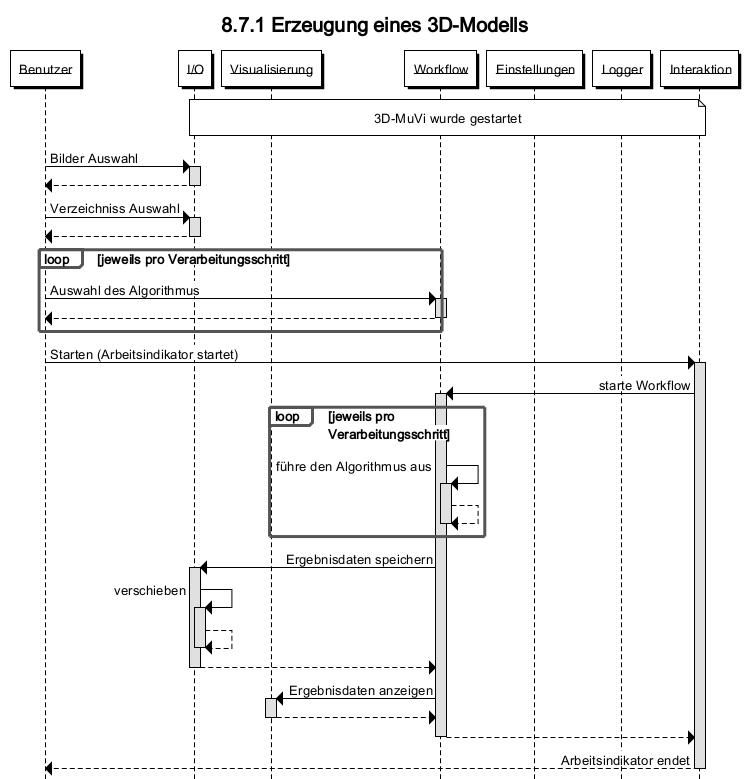
\includegraphics[width=1.05\textwidth]{img/871_Seqz.png} 

\section{Evaluierung von Algorithmen für Feature Extraktion / Matching}
\label{TNEvalAlgo}
\textbf{Vorbedingung:} Bilder eines Modells wurden erstellt. \newline
\textbf{Ergebnis:} Der Nutzer kann anhand der visuellen Betrachtung der Resultate einschätzen, welcher der beiden getesteten Algorithmen sich für die gewählten Bilder besser eignet. \newline
Der Nutzer führt folgende Schritte aus (Alle Schritte ab \ref{TNEvalAlgoBilderAuswahl} werden in 3D-MuVi ausgeführt):
\begin{enumerate}
	\item 3D-MuVi wird gestartet.
	\item \label{TNEvalAlgoBilderAuswahl} Bilder werden ausgewählt.
	\item Algorithmen für die folgenden Verarbeitungsschritte werden jeweils nacheinander ausgewählt:
	\begin{itemize}
		\item Feature Extraktion / Matching
		\item Posenschätzung
		\item Tiefenschätzung
		\item 3D Fusion
	\end{itemize}
	\item Button zum Starten der Verarbeitung wird gedrückt.
	\item Betrachtung der Ergebnisse.
	\item Anderer Algorithmus für den Verarbeitungsschritt Feature Extraktion / Matching wird ausgewählt.
	\item Button zum Starten der Verarbeitung wird gedrückt.
	\item Erneute Betrachtung der Ergebnisse.
\end{enumerate}
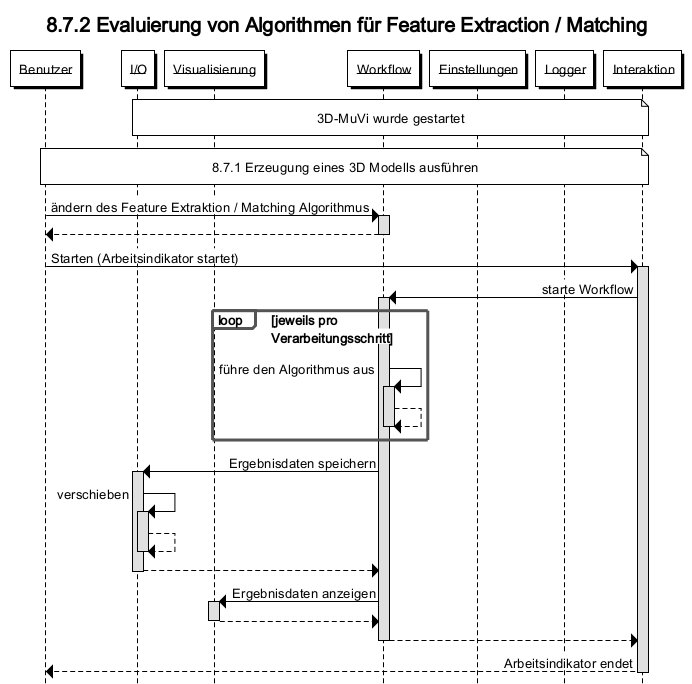
\includegraphics[width=1.05\textwidth]{img/872_Seqz.png}

\section{Überprüfen des Logs von Algorithmen}
\textbf{Vorbedingung:} Bilder eines Modells wurden erstellt. \newline
\textbf{Ergebnis:} Der Nutzer kann anhand der Meldungen im Log die Eignung der gewählten Algorithmen für die Bilder einschätzen und Verbesserungen an den Algorithmen vornehmen. \newline
Der Nutzer führt folgende Schritte aus (Schritte \ref{TNLogBilderAuswahl} bis \ref{TNLogSuchen} werden in 3D-MuVi ausgeführt):
\begin{enumerate}
	\item 3D-MuVi wird gestartet.
	\item \label{TNLogBilderAuswahl} Bilder werden ausgewählt.
	\item Algorithmen für die folgenden Verarbeitungsschritte werden jeweils nacheinander ausgewählt:
	\begin{itemize}
		\item Feature Extraktion / Matching
		\item Posenschätzung
		\item Tiefenschätzung
		\item 3D Fusion
	\end{itemize}
	\item Button zum Starten der Verarbeitung wird gedrückt.
	\item Alle Arten von Meldungen im Log werden eingeblendet.
	\item \label{TNLogSuchen} Auffälligkeiten in den Meldungen des Logs werden gesucht.
	\item Algorithmen werden bei Bedarf überarbeitet.
\end{enumerate}
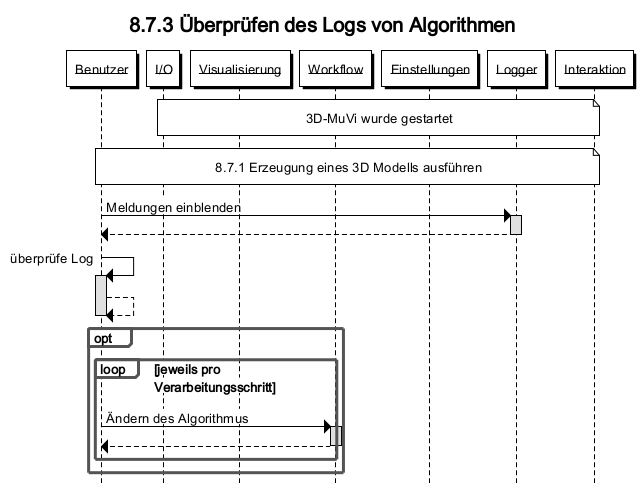
\includegraphics[width=1.05\textwidth]{img/873_Seqz.png}

\section{Evaluierung eines Workflows nach Entfernung eines Features in den Zwischenergebnissen}
Dieser Nutzungsablauf ist eine Erweiterung von \ref{TNEvalAlgo}. Sinn der Erweiterung ist es, dem Nutzer die Möglichkeit zu geben, das Entfernen einzelner Features zu testen, bevor er den Algorithmus entsprechend anpasst. Als optionale Funktion muss das Löschen einzelner Features in den Zwischenergebnissen und das Starten ab einem bestimmten Schritt implementiert sein. \newline
\textbf{Vorbedingung:} Bilder eines Modells wurden erstellt. \newline
\textbf{Ergebnis:} Der Nutzer kann anhand der visuellen Betrachtung der Resultate einschätzen, ob das Entfernen des Features das Endergebnis verbessert oder verschlechtert. Auf dieser Grundlage kann er über weitere Anpassungen an dem gewählten Algorithmus für die Feature Extraktion nachdenken. \newline
Der Nutzer führt folgende Schritte aus (Alle Schritte ab \ref{TNOFeatureEntfBilderAuswahl} werden in 3D-MuVi ausgeführt):
\begin{enumerate}
	\item 3D-MuVi wird gestartet.
	\item \label{TNOFeatureEntfBilderAuswahl} Bilder werden ausgewählt.
	\item Algorithmen für die folgenden Verarbeitungsschritte werden jeweils nacheinander ausgewählt:
	\begin{itemize}
		\item Feature Extraktion / Matching
		\item Posenschätzung
		\item Tiefenschätzung
		\item 3D Fusion
	\end{itemize}
	\item Button zum Starten der Verarbeitung wird gedrückt.
	\item Betrachtung der Ergebnisse.
	\item In den Ergebnissen der Feature Extraktion wird ein Feature entfernt.
	\item Button zum Starten der Verarbeitung ab dem Schritt Posenschätzung wird gedrückt.
	\item Erneute Betrachtung der Ergebnisse.
\end{enumerate}
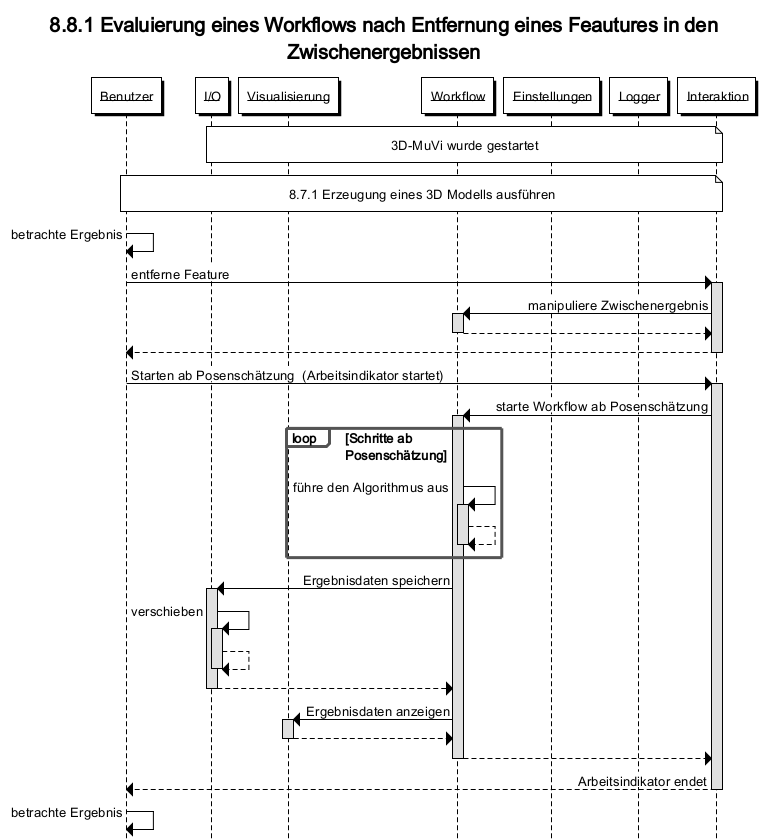
\includegraphics[width=1.05\textwidth]{img/881_Seqz.png}

\subsection{Evaluierung von Algorithmen für Feature Extraktion / Matching auf mehreren Datensätzen}
Dieser Nutzungsablauf ist eine Erweiterung von \ref{TNEvalAlgo}. Sinn der Erweiterung ist es, dem Nutzer die Möglichkeit zu geben, Workflows schnell auf mehreren Sätzen von Bildern zu evaluieren. Als optionale Funktion muss das Erstellen und Auswählen mehrerer Datensätze umgesetzt sein.\newline
\textbf{Vorbedingung:} Bilder zweier Modelle wurden erstellt (nachfolgend als Modell1 und Modell2 bezeichnet). \newline
\textbf{Ergebnis:} Der Nutzer kann anhand der visuellen Betrachtung der Resultate einschätzen, welcher der beiden getesteten Algorithmen sich für die gewählten Bilder von Modell1 bzw. Modell2 besser eignet. \newline
Der Nutzer führt folgende Schritte aus (Alle Schritte ab \ref{TNOEvalAlgoBilderAuswahl1} werden in 3D-MuVi ausgeführt):
\begin{enumerate}
	\item 3D-MuVi wird gestartet.
	\item \label{TNOEvalAlgoBilderAuswahl1} Bilder von Modell1 werden ausgewählt.
	\item Algorithmen für die folgenden Verarbeitungsschritte werden jeweils nacheinander ausgewählt:
	\begin{itemize}
		\item Feature Extraktion / Matching
		\item Posenschätzung
		\item Tiefenschätzung
		\item 3D Fusion
	\end{itemize}
	\item Button zum Starten der Verarbeitung wird gedrückt.
	\item Betrachtung der Ergebnisse.
	\item Neuer Datensatz für Modell2 wird erstellt und ausgewählt.
	\item Bilder von Modell2 werden ausgewählt.
	\item Button zum Starten der Verarbeitung wird gedrückt.
	\item Betrachtung der Ergebnisse.
	\item Anderer Algorithmus für den Verarbeitungsschritt Feature Extraktion / Matching wird ausgewählt.
	\item Button zum Starten der Verarbeitung wird gedrückt.
	\item Betrachtung der Ergebnisse.
	\item Datensatz von Modell1 wird gewählt.
	\item Betrachtung der Ergebnisse.
\end{enumerate}
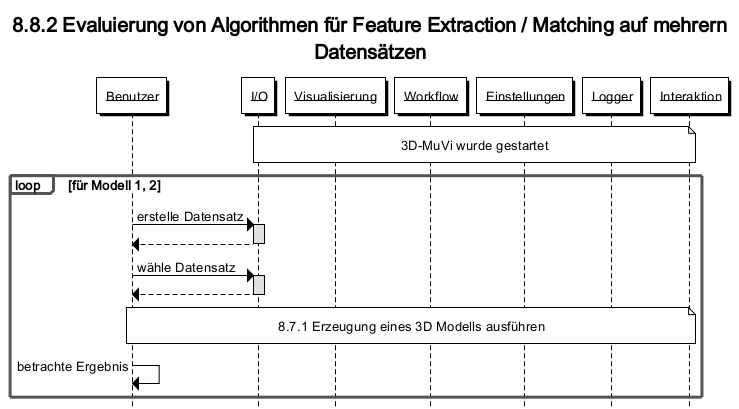
\includegraphics[width=1.05\textwidth]{img/882_Seqz.png}

\section{Aufgetretene Fehler}
\section{Codeüberdeckung}